\section{Collaborative ML Workload Optimizations} \label{sec-ml-workloads}
In this section, we provide an overview of of our collaborative ML workload optimization system.
Figure \ref{system-workflow} shows the high-level architecture of our system.
In a typical collaborative environment, users fetch datasets from a central server, perform their analysis on their local machine, and optionally store their results back in the central server.
Our system also comprises of a client and server.
The client is responsible for parsing user scripts into workload DAGs.
The server receives the workload DAGs and returns an optimal execution DAG.
Finally, the client executes the optimal execution DAG and prompts the materializer component to update the Experiment Graph.
%The client supports both python scripts and interactive Jupyter notebooks.
%The client is also responsible for executing a given workload.
%The Experiment Graph resides on the server side, which enables workload optimization through materialization and reuse of ML artifacts.
%After the optimization, the client receives the optimized program and executes it locally.
This architecture enables us to integrate to existing collaborative environment without requiring any changes to the current workflow of the collaborative environments.
In the rest of this section, we first describe the process of parsing and executing workloads.
Then, we describe the process of optimizing workloads and materializing workloads into the Experiment Graph.
Finally, we address the integration process and the impact of our system on the use case in Section \ref{subsec-motivational-example}.

\begin{figure}
\centering
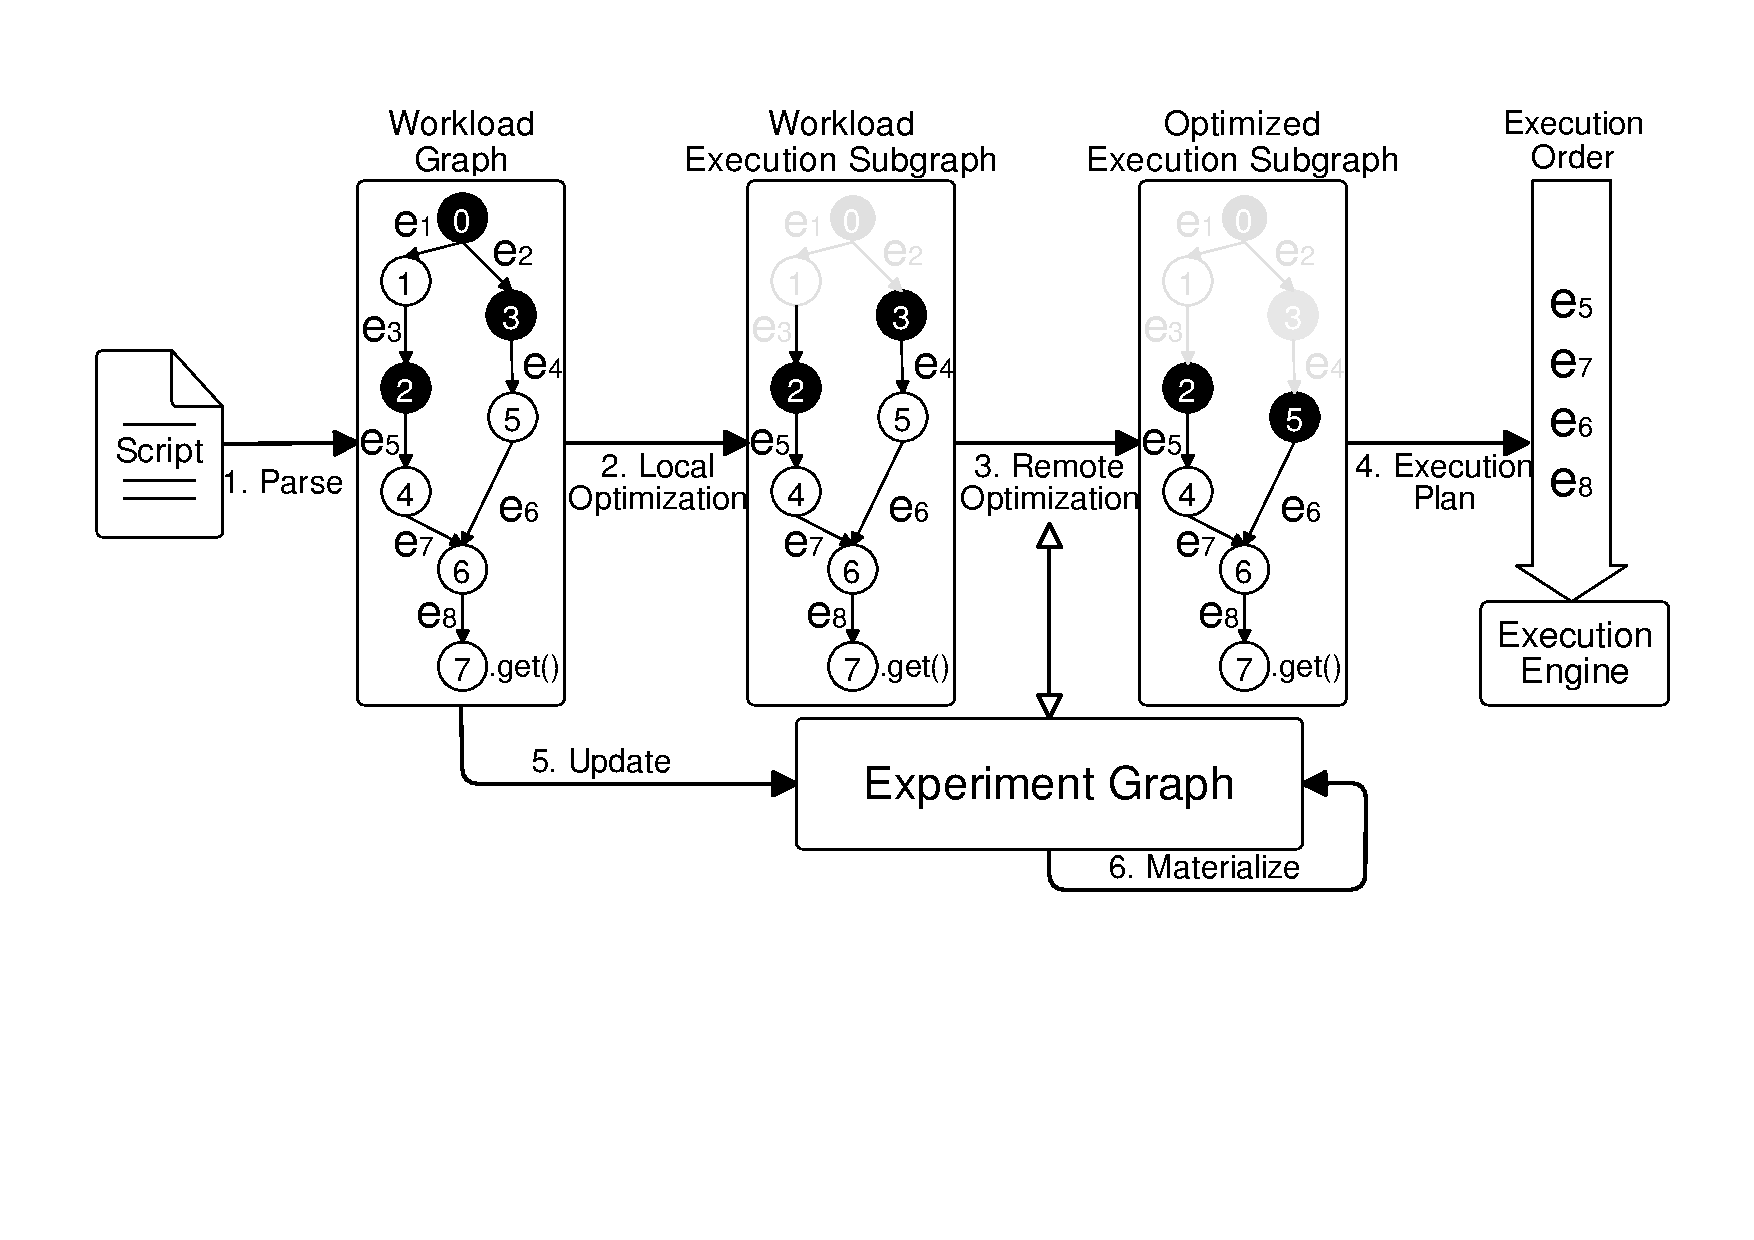
\includegraphics[width=0.7\columnwidth]{../images/system-workflow}
\caption{System overview of the collaborative workload optimizer}
\label{system-workflow}
\end{figure}

\subsection{Workload Parsing and Execution}
\textbf{ML Script Parsing.}
Instead of designing a new DSL, we extend the existing Pandas and scikit-learn \cite{sklearn_api} python packages that are frequently used for data analysis and machine learning workloads.
Listing \ref{listing-experiment-graph} shows an example of a workload script.
With only a slight modification of the import commands, we are able to load our system's modules.
As a result, we support both python scripts and interactive Jupyter notebooks.
Listing \ref{listing-experiment-graph} shows an example of a script.
\begin{lstlisting}[language=Python, caption=Example script,captionpos=b,label = {listing-experiment-graph}]
import custom_pandas as pd

from custom_sklearn import svm
from custom_sklearn.feature_selection import SelectKBest
from custom_sklearn.feature_extraction.text import CountVectorizer

train = pd.read_csv('../input/train.csv') 
print train.columns # [ad_desc,ts,u_id,price,y]
vectorizer = CountVectorizer()
count_vectorized = vectorizer.fit_transform(train['ad_desc'])
selector =  SelectKBest(k=2)
top_features = selector.fit_transform(
                                  train[['ts','u_id','price']],  
                                  train['y'])
top_features # print the content of the data frame			     
X = pd.concat([count_vectorized,top_features], axis = 1)
model = svm.SVC().fit(X, train['y'])
model.get() # terminal vertex
\end{lstlisting}

\textbf{Workload DAG.}
A machine learning workload can be represented using a directed acyclic graph (DAG).
In our DAG representation, vertices represent the artifacts, i.e., raw or preprocessed data (represented by data frame objects) and machine learning models resulting from feature engineering and model training operations and edges represent the operations in the workload.
Each workload DAG has one or more initial vertices representing the raw datasets which are defined as part of the task definition in a collaborative platform.
We refer to the initial vertices as the sources.
The parser component, step 1 in Figure \ref{system-workflow}, reads the user script and generates the workload DAG.
Figure \ref{fig-experiment-graph}a shows an example DAG constructed from the code in Listing \ref{listing-experiment-graph}.
\begin{figure}
\centering
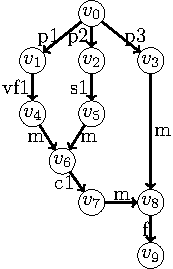
\includegraphics[width=0.8\linewidth]{../images/tikz-standalone/example-graph}
\caption{Experiment graph constructed from the Listing \ref{listing-experiment-graph} (a) and the hash of the operations in the scripts (b)}
\label{fig-experiment-graph}
\end{figure}
Table \ref{fig-experiment-graph}b shows both the label of every edge operation, i.e., time, and the hash of the operations and their hyperparameters.

\textbf{Experiment Graph. }
For every task, the collection of all the DAGs of the previously executed machine learning workloads forms a rooted graph (with potentially multiple root vertices) which we refer to as the \textit{experiment graph}.
More formally, we represent the experiment graph by $G(V, E)$.
$V=\{v_i\}, i = 1, \cdots, n$ is the set of all the artifacts in all the workload DAGs.
$E=\{e_i\}, i = 1, \cdots, m$ is the set of all the executed operations in the workload DAGs.
A directed edge $e$ from $v_i$ to $v_j$ in $G(V, E)$ indicates that the artifact $v_j$ is derived from the artifact $v_i$ by applying the operation in $e$.
Every vertex $v$ has the attributes $\langle f, s \rangle$ (accessed by $v.f$ and $v.s$) which represent the frequency, i.e., number of different workloads an artifact appeared in, and storage size of the artifact.
Every edge $e$ has the attribute $\langle t \rangle$ (accessed by $e.t$) which represents the run-time (in seconds) of the operation.

Inside each vertex, we store the meta-data of the artifact.
Depending on how \textit{useful} an artifact is, we may also store the actual underlying data inside the artifact (Section \ref{sec-materialization}).
If the artifact is a raw or a preprocessed dataset, then its meta-data includes the name, type, and total size of each column of the data and its underlying data is represented by the dataframe object (i.e., Pandas dataframe). 
If the artifact is a machine learning model, its meta-data includes the name, type, hyperparameters, and the error metric of the model and its underlying data is consist of the model weights.
Each edge contains the meta-data of the operation it represents, such as the function name, training algorithm, and hyperparameters.
To uniquely identify an edge, we utilize a hash function which receives as input the operation and its hyperparameters (if it has any).
Since the experiment graph is rooted, we assign a hash value to every vertex which is computed in the following way:
\[
    h(v)= 
\begin{cases}
    id,& \text{if } v \text{ is root}\\
    h\Big(\sum\limits_{e \in in\_edge(v)} (h(e.source) + h(e) ) \Big)  ,              & \text{otherwise}.
\end{cases}
\]
where $in\_edge(v)$ returns the edges with destination $v$. 
Intuitively, the hash of a root vertex is its unique identifier (location on disk or download URL) and the hashes of other vertices are derived recursively by combining the hashes of their parents and edges which connect them to their parents.

After a machine learning workload is executed, we update the experiment graph by adding the new artifacts and operations.
If any of the artifacts already exist in the graph, their frequency is updated.





We start with an empty Experiment Graph.
After the execution of the script and updating the Experiment Graph, all the artifacts (vertices) have a frequency of 1.
To represent operations which process multiple input artifacts, e.g., concat and svm.fit operations in Listing \ref{listing-experiment-graph}, we proceed as follows.
First, we merge the vertices representing the artifacts into a single vertex using a merge operator.
The merge operator is a logical operator which does not incur a cost, i.e., it has a run-time of 0 seconds.
The merged vertex is also a logical vertex with no actual attributes which only contains the vertex ids of the merged vertices.
Then, we draw an edge from the merged vertex which represents the actual operation.
For example, in Figure \ref{fig-experiment-graph}a, before applying the concatenation operation, we merge $v_4$ and $v_5$ into $v_6$, then we apply the concatenation operation (c1).
Furthermore, when computing the hash of a merged vertex, we take the merge order into account.
For example, the operation svm.fit has $X$ (represented by $v_7$) as first argument and train['y'] (represented by $v_3$) as its second argument.
When computing hash of $v_8$, we combine the parents in the same order, i.e., $h(v_8) = h(h(v_7) + m + h(v_3) + m)$. 
After the DAG is constructed, its execution is invoked with the call to the $get()$ command on Line 18.

\subsection{System Architecture and Workflow}
Figure \ref{system-workflow} shows the components of our collaborative workload optimizer system.
First, a parser component generates the workload DAG from the user scripts (Step 1).
Upon the invocation of the $get()$ method of a vertex, i.e., the terminal vertex, a local optimization process beings.
The local optimizer extracts the subgraph which must be executed in order to compute the terminal vertex.
The local optimizer traverses the graph in reverse order starting at the terminal vertex until the root vertices.
It stops the traversal when it reaches a previously computed vertex.
In interactive workloads, it is likely that many of the intermediate vertices between the terminal vertex and the root vertices are previously computed.
The subgraph of all the visited vertices and the edges connecting them is another DAG, which we refer to as the \textit{local execution DAG}, and is the result of the local optimizer (Step 2).
The global optimizer component receives the local execution DAG and looks for optimization opportunities, i.e., reusing materialized vertices or warmstarting model training, in the experiment graph.
Using early stopping, search space pruning, and heuristics the global optimizer finds the relevant artifacts \hl{with negligible overhead}.
The result of the global optimization process is another subgraph, which we refer to as the \textit{global execution DAG} (Step 3).
Then, an execution planner receives the global execution DAG and generates the execution schedule by sorting the edges based on their topological order, which is then executed by the execution engine (Step 4).
If the experiment graph is empty, then the execution planner users local execution DAG to generate the execution schedule.
After the execution, an updater component updates the experiment graph to include the vertices and edges of the workload DAG (Step 5).
Lastly, a materializer component decides what vertices to materialize, i.e., store their underlying data in the vertex of the graph (Step 6).


\subsection{Improved Use Case}
In this section, we show how our collaborative workload optimizer improves the workload execution process of the Kaggle use case we described in Section \ref{sec-background}.
For the Home Credit Default Risk competition, we maintain an Experiment Graph.
Before any workloads are executed, the Experiment Graph is empty.
Given an empty Experiment Graph, when users submit workloads for execution, our collaborative workload optimizer skips Step 3 of Figure \ref{system-workflow} and generates the execution plan directly from the workload execution subgraph.
We update the Experiment Graph with the DAG of incoming user workloads.
The materializer component decides what artifacts of incoming the user workloads to keep and what are artifacts to discard.
Since one criterion for selecting artifacts to materialize is execution frequency, the materializer selects the artifacts of the two popular workloads described in the use case for materialization.
For all the future workloads, the global optimizer, Step 3 of Figure \ref{system-workflow}, looks for reuse and warmstarting opportunities. 
As a result, our optimizer reduces the execution time of all the 6000 copied and edited versions of the two popular workloads. 
This reduces the required resources and operation cost of Kaggle.